%
        \section{Capacitively Coupled RF Discharges}
%   
			\begin{wrapfigure}[13]{r}{0.4\textwidth}
				\centering%
				\vspace*{-0.5cm}%
				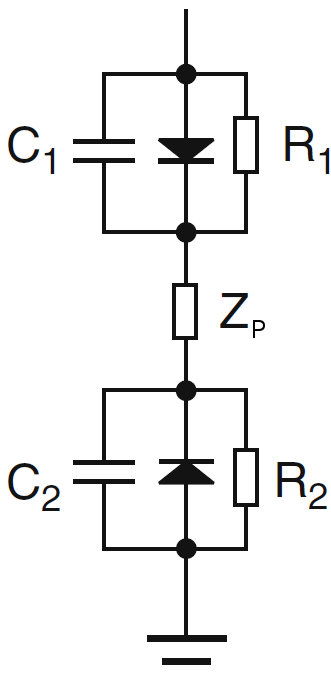
\includegraphics[width=0.17\textwidth]{figures/circuit_selfbias_piel.png}
				\caption{%
					Replacement circuit of an asymmetrically driven ccrf %
					discharge.~\cite{Piel10} A diode represents the directed electron %
					current from the sheaths $j=1,2$.}\label{fig:replacementcurrent}
			\end{wrapfigure}
%
           Most rf plasmas are asymmetric discharges due to the contact of the ionized gas with the vacuum vessel. The asymmetry characterised by the area ratio of driven electrodes and grounded walls. A step towards the characterisation of asymmetric ccrf discharges is the development of a replacement circuit, see~\autoref{fig:replacementcurrent}. Thus, one can define a specific impedance for a rf discharge of excitation frequency $\omega$. The value of $\varepsilon\ix{p}$ resembles the permeability of the working gas between the driven and/or grounded electrode~\cite{Piel10}. In addition, this volume has the capacity $C\ix{p}$ --- the capacity of a cubicle with a cross section $A$, thickness $b$ and electron-neutral collision frequency $\nu\ix{e,n}$ calculates like~\autoref{equ:capacityandepsilon}.
%
				\begin{align}
					\varepsilon\ix{p}=&1-\frac{\omega\ix{p,e}^2}{\omega\left(\omega-\imag\nu\ix{e,n}\right)}\,,%
						\quad\quad%
						C\ix{p}=\varepsilon\ix{p}C\ix{0}=%
						\varepsilon\ix{p}\varepsilon\ix{0}\frac{A}{b}%
						\label{equ:capacityandepsilon}\\[0.2cm]
					&Z\ix{p}={\left(\imag\omega C\ix{p}+ \frac{1}{\frac{1}{\omega\ix{p,e}^2C\ix{0}}%
							{\left(\nu\ix{e,n}+\imag\omega\right)}}\right)}^{-1}%
					\label{equ:bulkimpedanz}
				\end{align}
%		
				The~\autoref{equ:bulkimpedanz} represents the full electrical impedance, consisting of the inverse sum of real and imaginary resistance, as well as the capacity of the neutral gas volume. Here, $\imag\omega/(\omega\ix{p,e}^{2}C\ix{0})$ characterizes the electrons inertia in regard to an external excitation $\omega$. The real part $\nu\ix{e,n}/(\omega\ix{p,e}^{2}C\ix{0})$ denotes the resistance by neutral particle collisions. For high excitation frequencies, e.g.\@ $\SI{13.56}{\mega\hertz}$ the bulk impedance can be neglected (see~\autoref{equ:bulkimpedanz}~\cite{Kay85}). Both sheath capacities of anode and cathode take the dominant part.
%
            \subsection{Self Bias Voltage}\label{sec:selfbias}
%            
				The plasma potential $\Phi\ix{p}(t)$ and voltage across the discharge $U(t)$ can be written as:
%
				\begin{align}
					U\left(t\right)=U\ix{sb}+U\ix{rf}\sin\left(\omega t\right)%
%						\nonumber\\[0.0cm]
						\quad\text{~and~}\quad%
						\Phi\ix{p}\left(t\right)=\overline{\Phi\ix{p}}+%
						\Phi\ix{rf}\sin\left(\omega t\right)\,.%
						\label{equ:selfbias_1}
				\end{align}
%
				Both sheaths of the electrodes collapse completely during a full cycle of $U(t)$. At this moment no potential barrier or space charge is hindering the particles to hit the electrodes. Electrons and ions can impinge on the surface and force the plasma potential $\Phi\ix{P}$ to level out with the walls. This short circuit between plasma and sheath occurs when $\Phi\ix{P}$ becomes negative with regard to the excitation ---~\autoref{equ:selfbias_unequal} and~\autoref{fig:circuitselfbias_2} express this circumstance:
%
				\begin{align}
					\Phi_{\text{p},\max}=\overline{\Phi\ix{p}}+\Phi\ix{rf}\geq U\ix{sb}+U\ix{rf}\,,%
%						\nonumber\\[0.0cm]
						\quad\quad%
						\Phi_{\text{p},\min}=\overline{\Phi\ix{p}}-\Phi\ix{rf}\geq0%
						\label{equ:selfbias_unequal}
				\end{align}
%
				\begin{figure}[!t]
					\centering%
					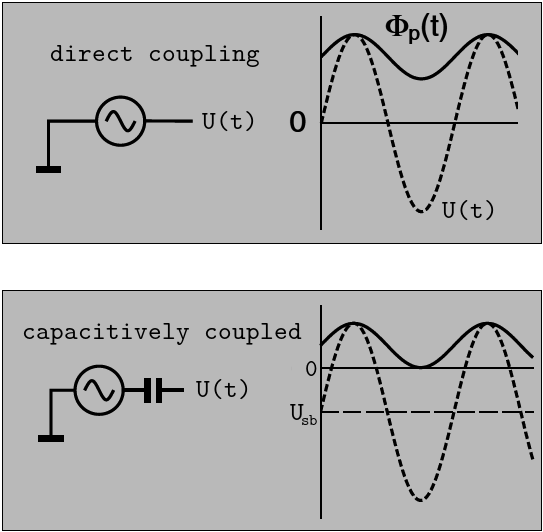
\includegraphics[width=0.95\textwidth]{figures/selfbiasvoltage.png}
					\caption{%
						Schematics of the voltage $U(t)$ and plasma potential $\Phi(t)$ %
						for a directly and capacitively coupled rf discharge. Different cases of %
						symmetry are shown: enlarged driven electron, grounded %
						electrode and a symmetric discharge.~\cite{Piel10}}\label{fig:circuitselfbias_2}
				\end{figure}
%
                A common approximation for the self bias voltage is roughly half of the driven electrodes peak-to-peak voltage: $|U\ix{sb}|\approx U\ix{rf}/2$.\\
				If there is no special coupling between electrode and electrical driver, the equality in~\autoref{equ:selfbias_unequal} is true. However, if a capacitive coupling is used, there can not be any net current between excitation and electrode because of charge conservation and current continutiy. The capacitance can not be inverted over the course of one rf cycle. The electron currents are then equal on both electrodes, therefore shifting the minimum plasma potential to ground and the maximum to the excitation.
				Finally, the dc \emph{self bias} part $U\ix{sb}$ and the mean plasma potential $\overline{\Phi\ix{p}}$ are:
%
				\begin{align}
					\overline{\Phi\ix{p}}=\frac{1}{2}(U\ix{sb}+U\ix{rf})\,,%
%						\nonumber\\[0.0cm]
                        \quad\text{~and~}\quad%
    					U\ix{sb}=\frac{C\ix{1}-C\ix{2}}{C\ix{1}+C\ix{2}}U\ix{rf}%
						\,\,.%
					\label{eq:selfbiaszwei} 
				\end{align}
%
				If the excitation frequency $\omega$ is small compared to other time scales, e.g\@ electron and ion plasma frequencies, the electron current from the sheath becomes bigger than the displacement current. Hence the electron current onto the driven electrode decreases by a Maxwell factor --- this is a function of the there-on applied voltage --- compared to the corresponding ion current. Therefore the sheaths impedance is bigger than those of the floating walls. Together with~\autoref{equ:selfbias_1} and~\autoref{equ:inequality} the plasma potential $\Phi\ix{p}$ vanishes and only the currents onto the driven electrode have to be equal. With $\mathbf{I}\ix{0}$ the zeroth order modified \emph{Bessel function} the following equation yields the self bias voltage:
%      
				\begin{align}
					U\ix{sb}=\frac{k\ix{B}T\ix{e}}{e}\ln%
						\left[\mathbf{I}\ix{0}\left(\frac{eU\ix{rf}}{k\ix{B}T\ix{e}}\right)\right]\,.%
					\label{equ:selfbias_3}
				\end{align}